\section{理論推導}

控制方程式與 SSSS 板完全相同，如式 \eqref{eq:gov}，差異僅在邊界條件。

\subsection{四邊固支邊界條件}
在所有四邊上，橫向位移與兩個轉角均為零：
\[
w = 0,\quad \phi_x = 0,\quad \phi_y = 0.
\]
由於邊界條件複雜，無法使用 Navier 級數分離變數求解。Reddy \cite{reddy2004} 在第 7.5 節中採用有限元法求解此問題，並以表格 (Table 7.5.1) 給出不同厚跨比下的無量綱屈曲係數。

\subsection{參考解與擬合公式}
對於四邊固支方板，第一模態的屈曲係數可擬合為：
\begin{equation}
\boxed{K_{\text{CCCC}} = \frac{10.31}{1 + 2.18\left(\dfrac{h}{b}\right)^2}} \label{eq:K_cccc}
\end{equation}
當 \(h\to 0\) 時，\(K\to 10.31\)，與經典薄板解一致。高階模態的參考值可採用文獻 \cite{leissa1969} 提供的古典解（薄板極限），或由極細網格數值解提供。

\section{數值模型}
與 SSSS 相同，但邊界罰函數須同時約束 \(w\)、\(\phi_x\)、\(\phi_y\)。懲罰係數 \(\alpha = 10^8 D\)。\textbf{網格劃分範圍亦為 \(n_{div} = 9\) 至 \(25\)，以進行收斂性研究。}

\section{結果與討論}
\subsection{屈曲模態圖}
圖 \ref{fig:cccc_modes} 顯示四邊固支板在 \(h=0.01\) 時的前六階屈曲模態，圖中座標軸 \(x, y\) 為板面內方向，顏色對應側向位移。

\begin{figure}[h!]
\centering
\begin{subfigure}{0.45\textwidth}
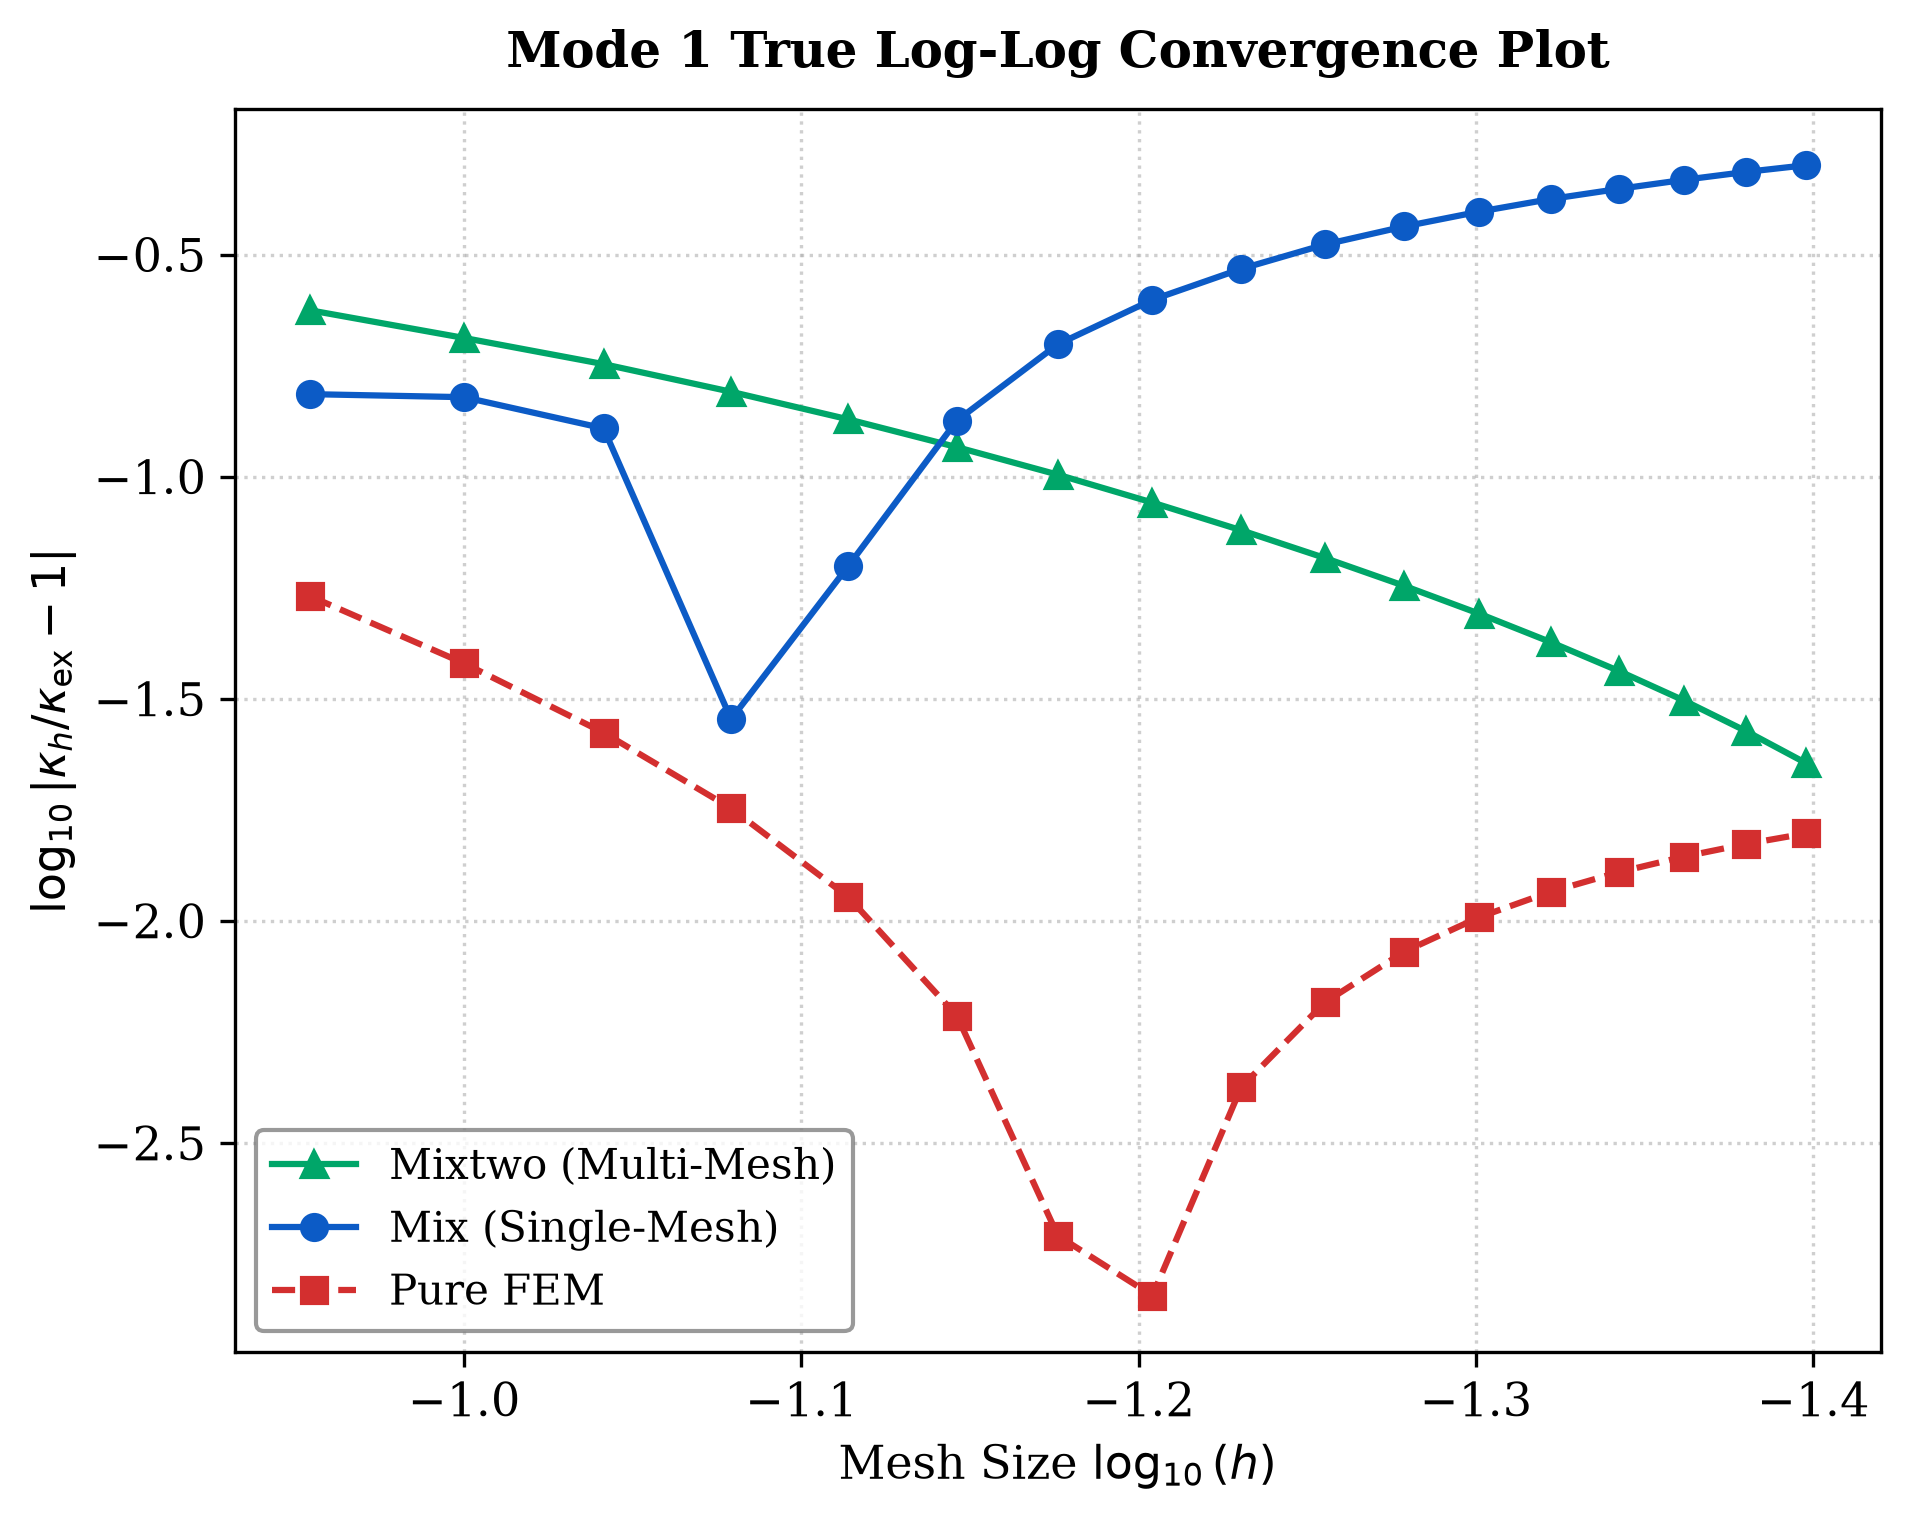
\includegraphics[width=\textwidth]{../images/buckling_mode_1_4c.png}
\caption{模態 1}
\end{subfigure}
\hfill
\begin{subfigure}{0.45\textwidth}
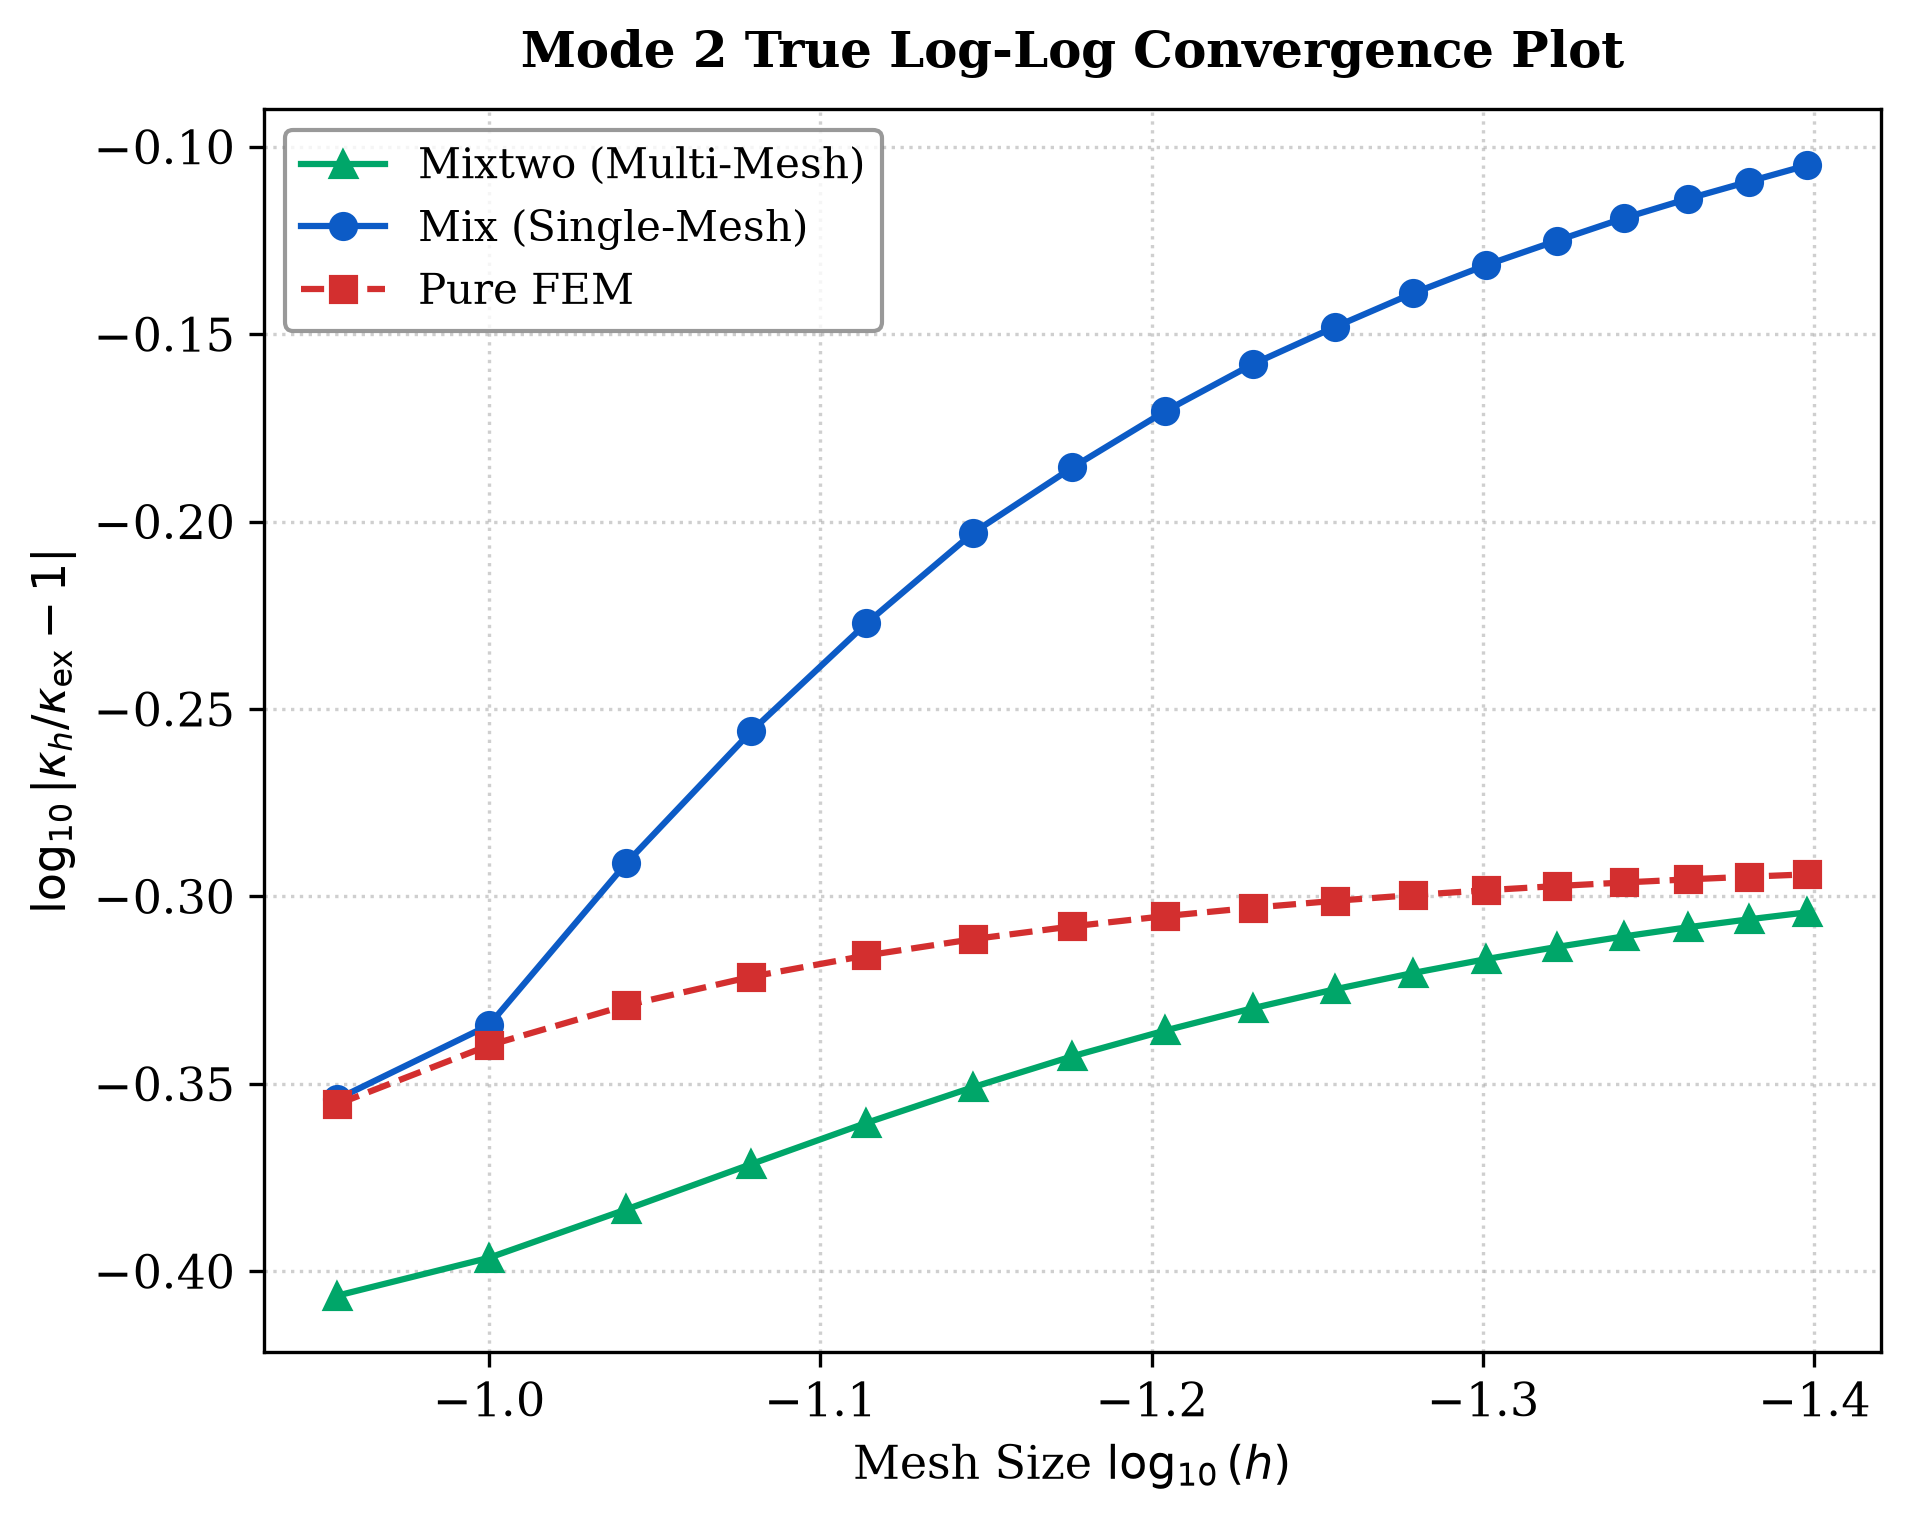
\includegraphics[width=\textwidth]{../images/buckling_mode_2_4c.png}
\caption{模態 2}
\end{subfigure}

\vspace{0.5cm}

\begin{subfigure}{0.45\textwidth}
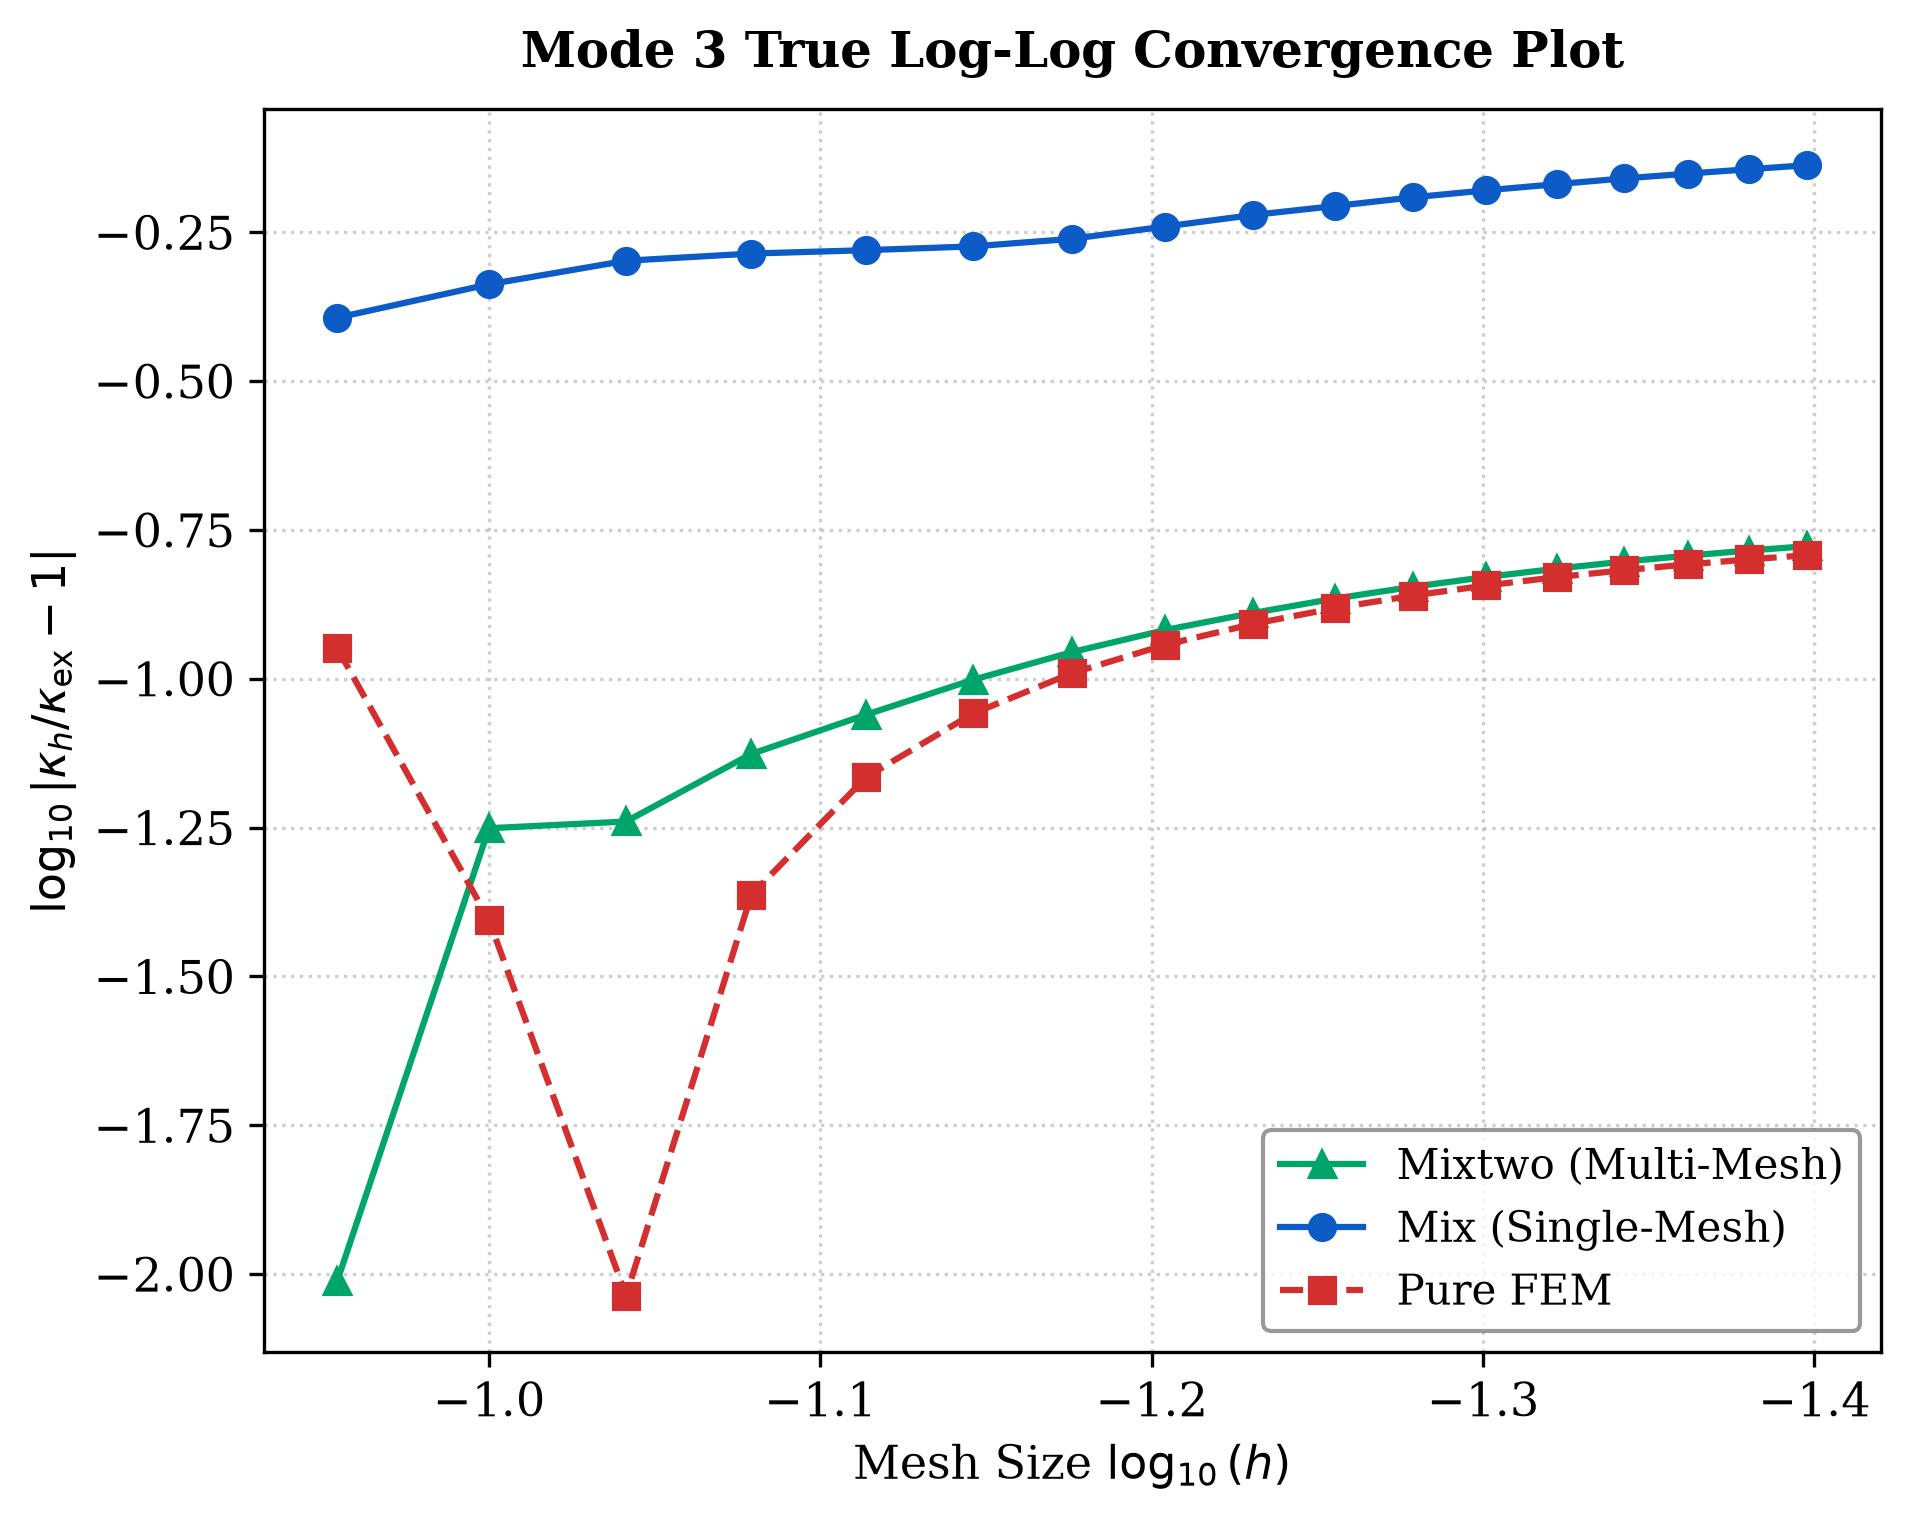
\includegraphics[width=\textwidth]{../images/buckling_mode_3_4c.png}
\caption{模態 3}
\end{subfigure}
\hfill
\begin{subfigure}{0.45\textwidth}
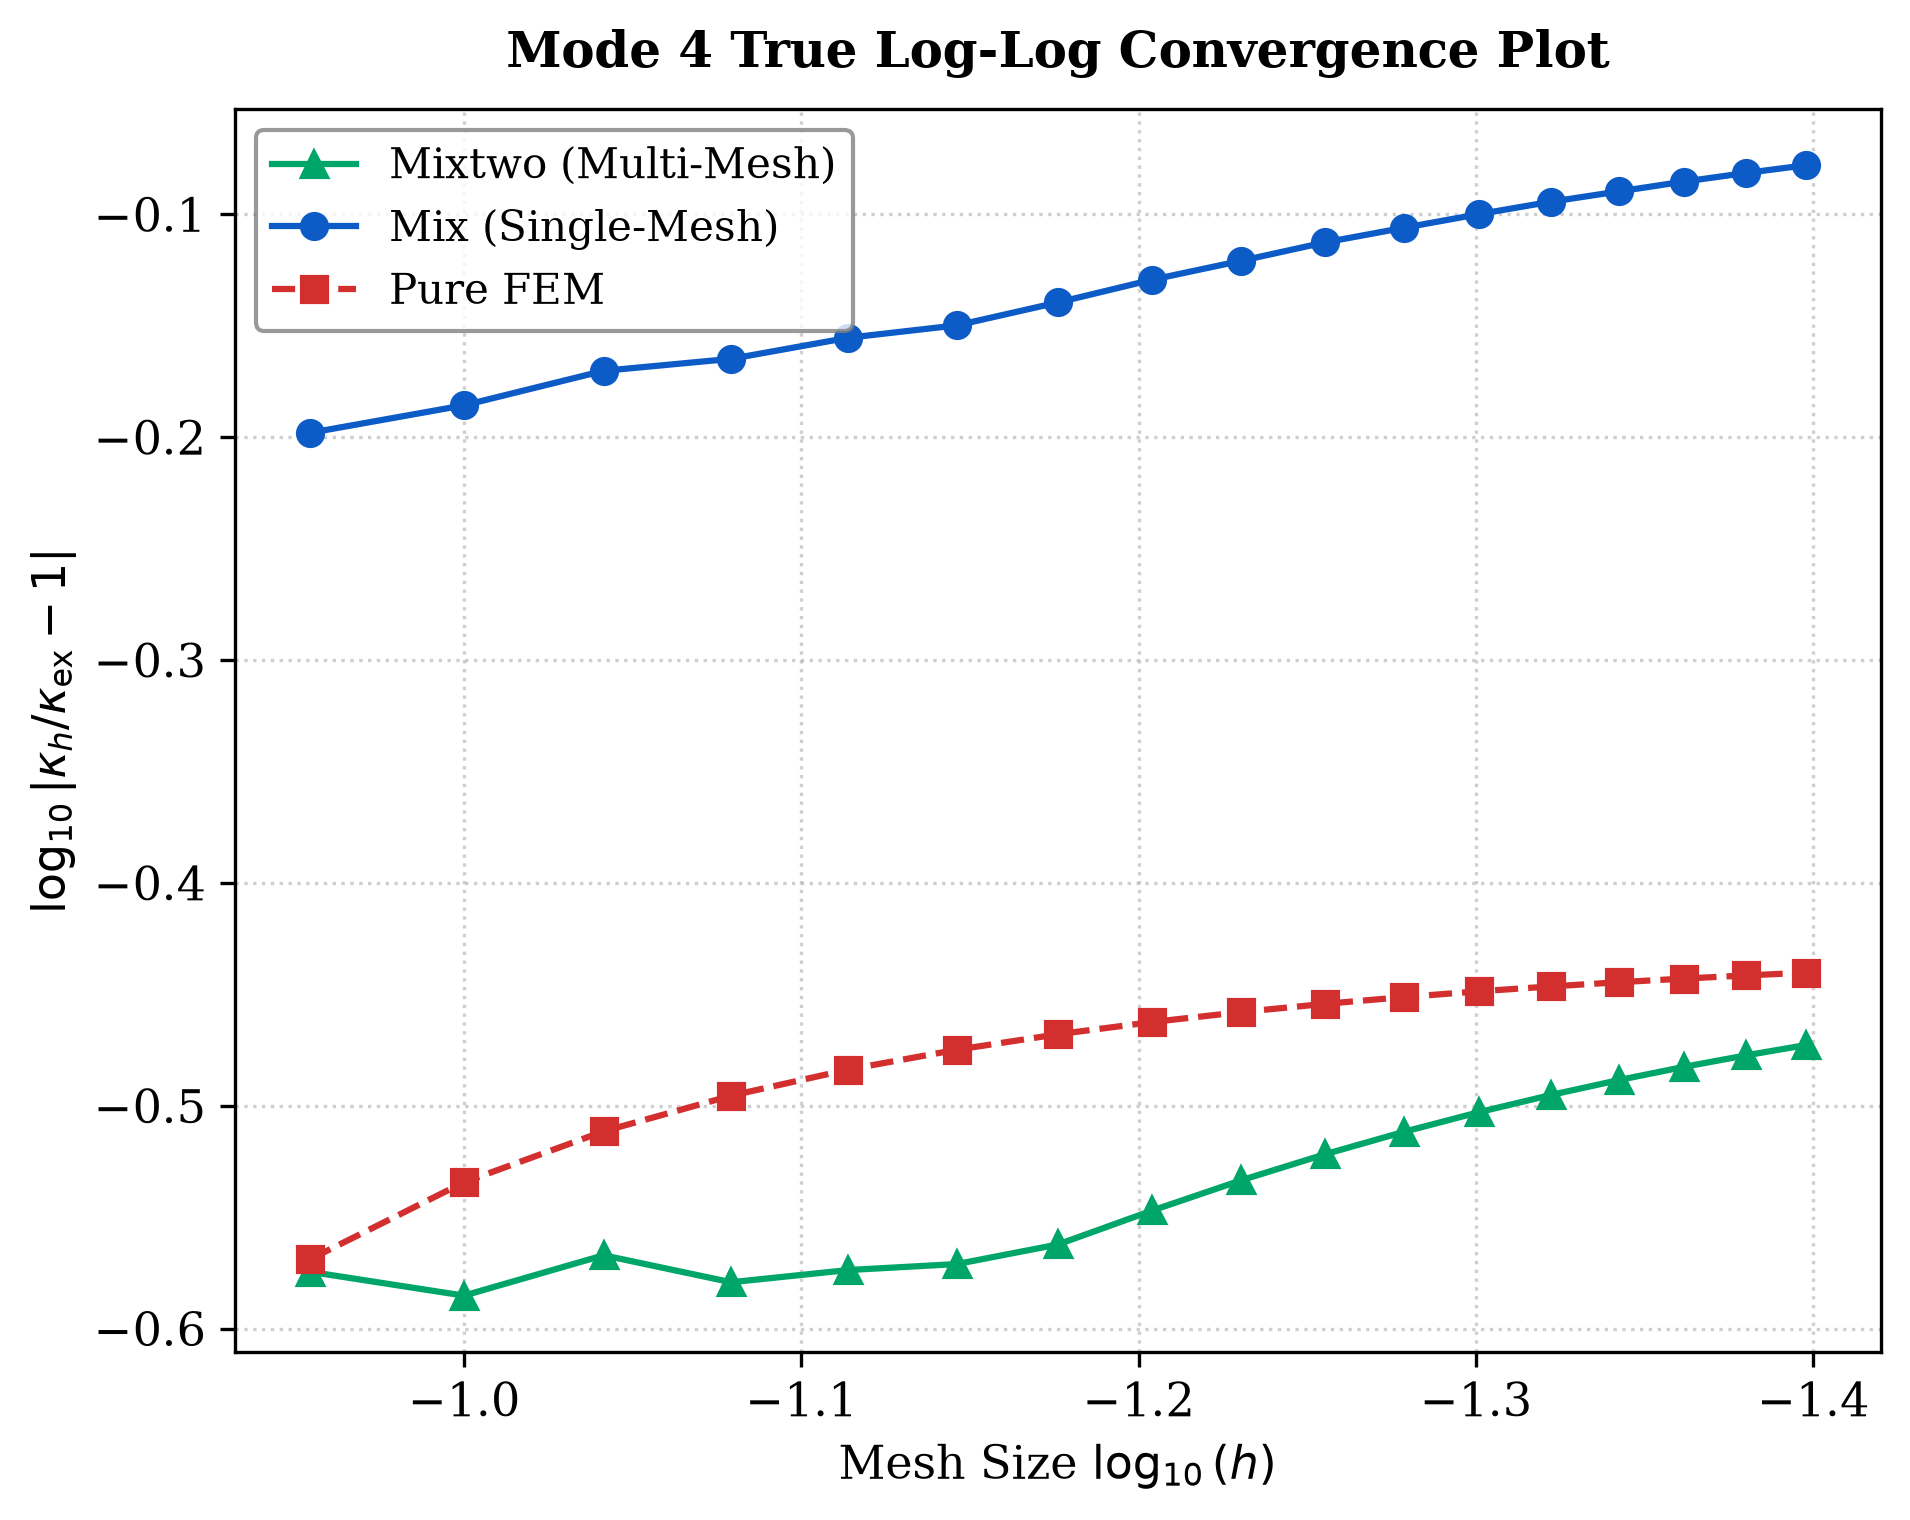
\includegraphics[width=\textwidth]{../images/buckling_mode_4_4c.png}
\caption{模態 4}
\end{subfigure}

\vspace{0.5cm}

\begin{subfigure}{0.45\textwidth}
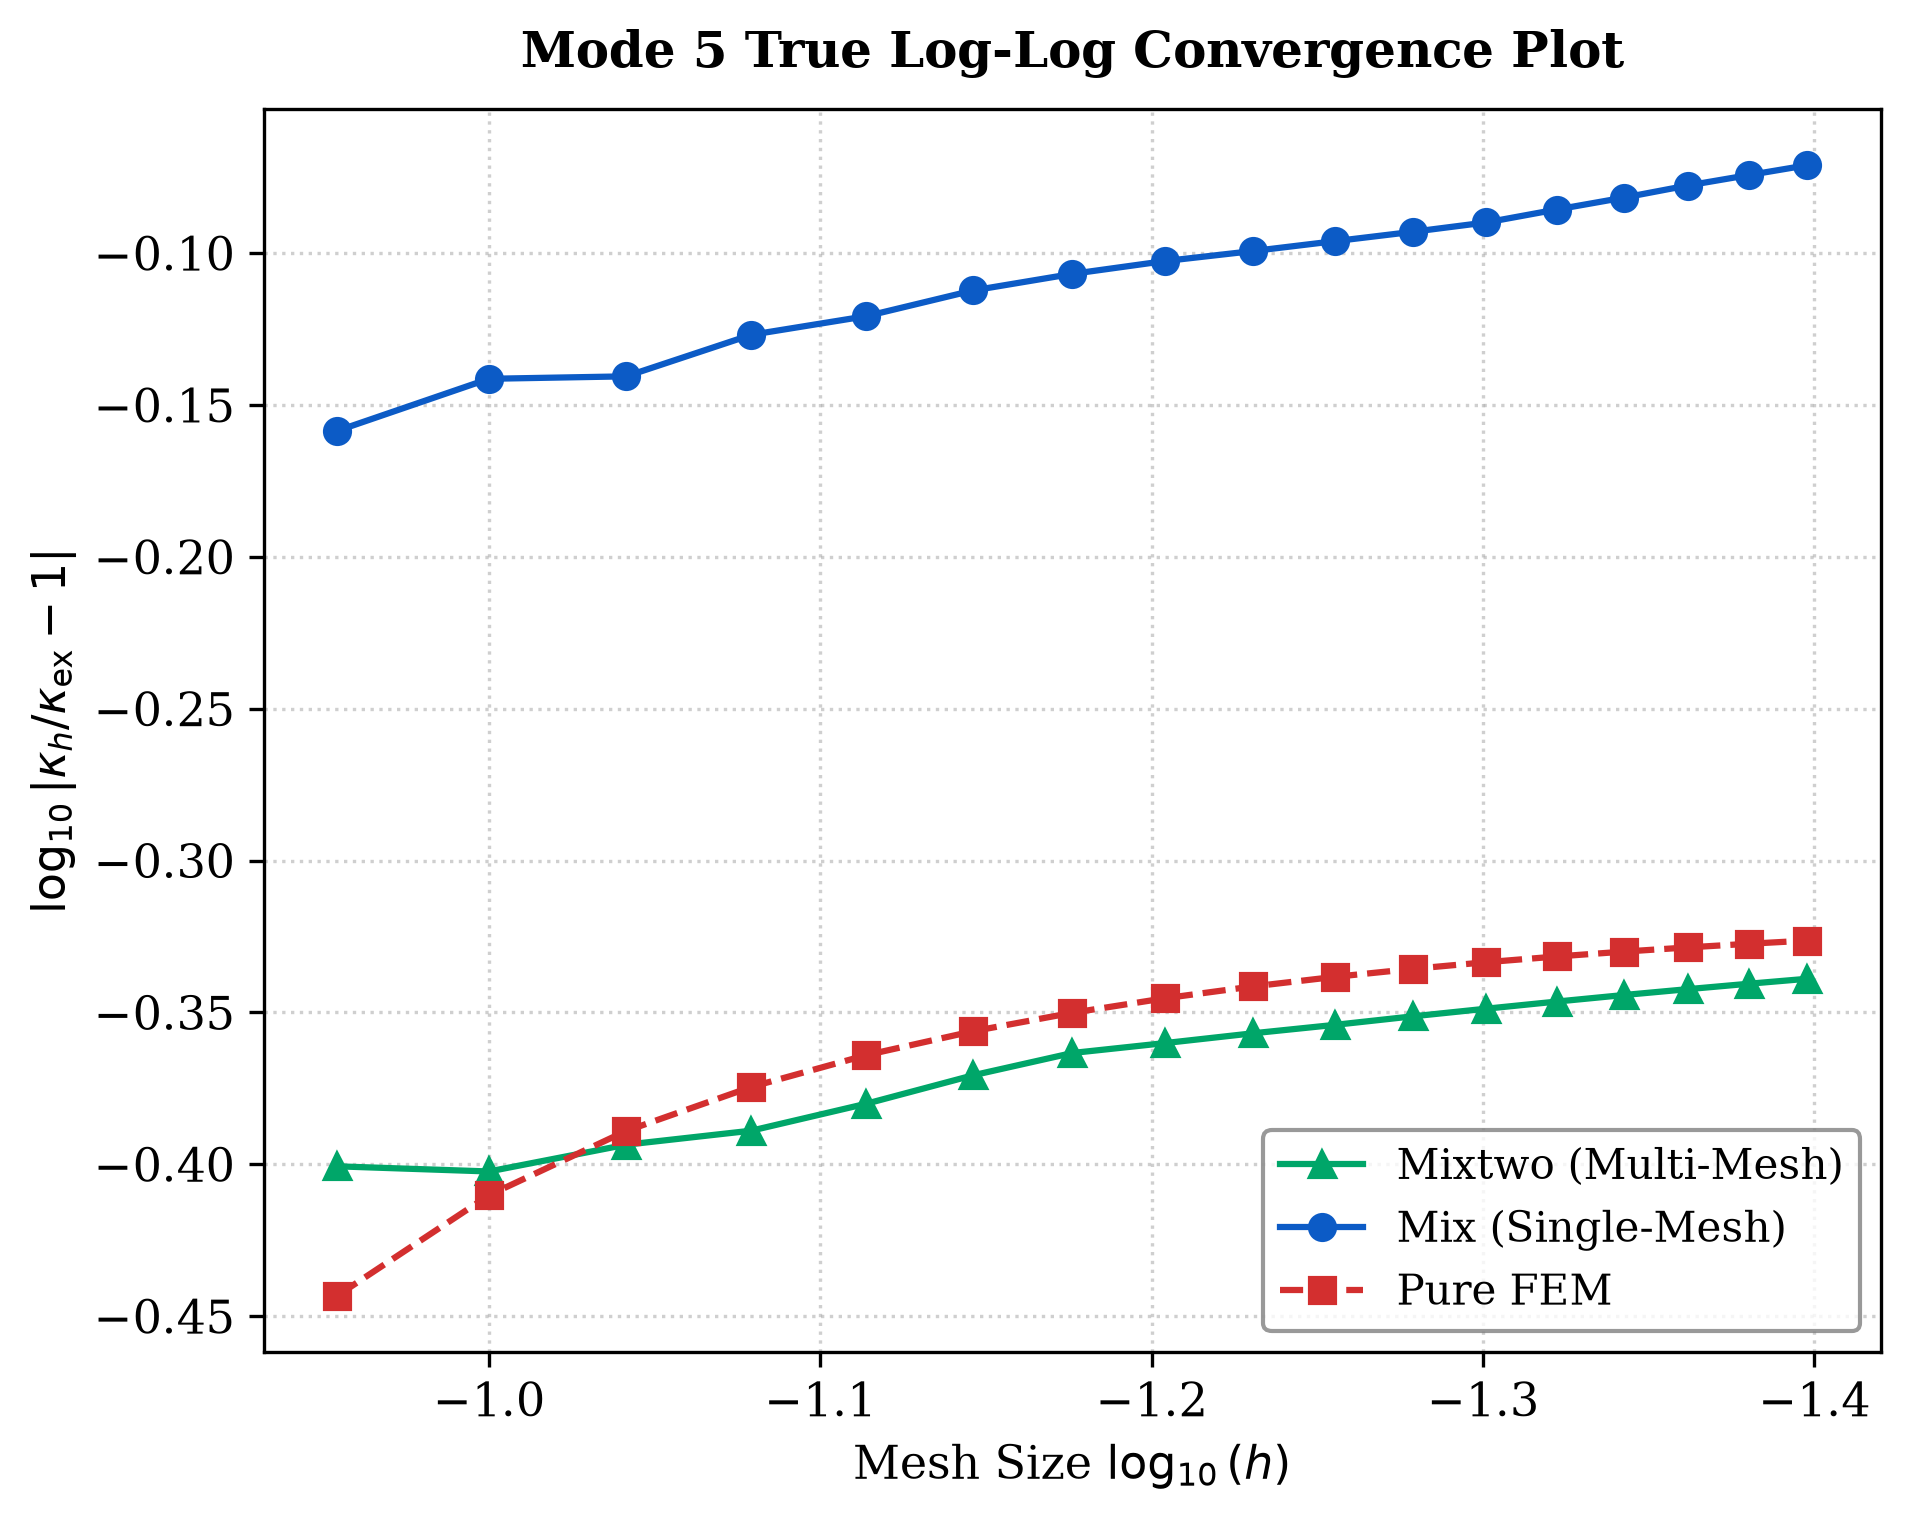
\includegraphics[width=\textwidth]{../images/buckling_mode_5_4c.png}
\caption{模態 5}
\end{subfigure}
\hfill
\begin{subfigure}{0.45\textwidth}
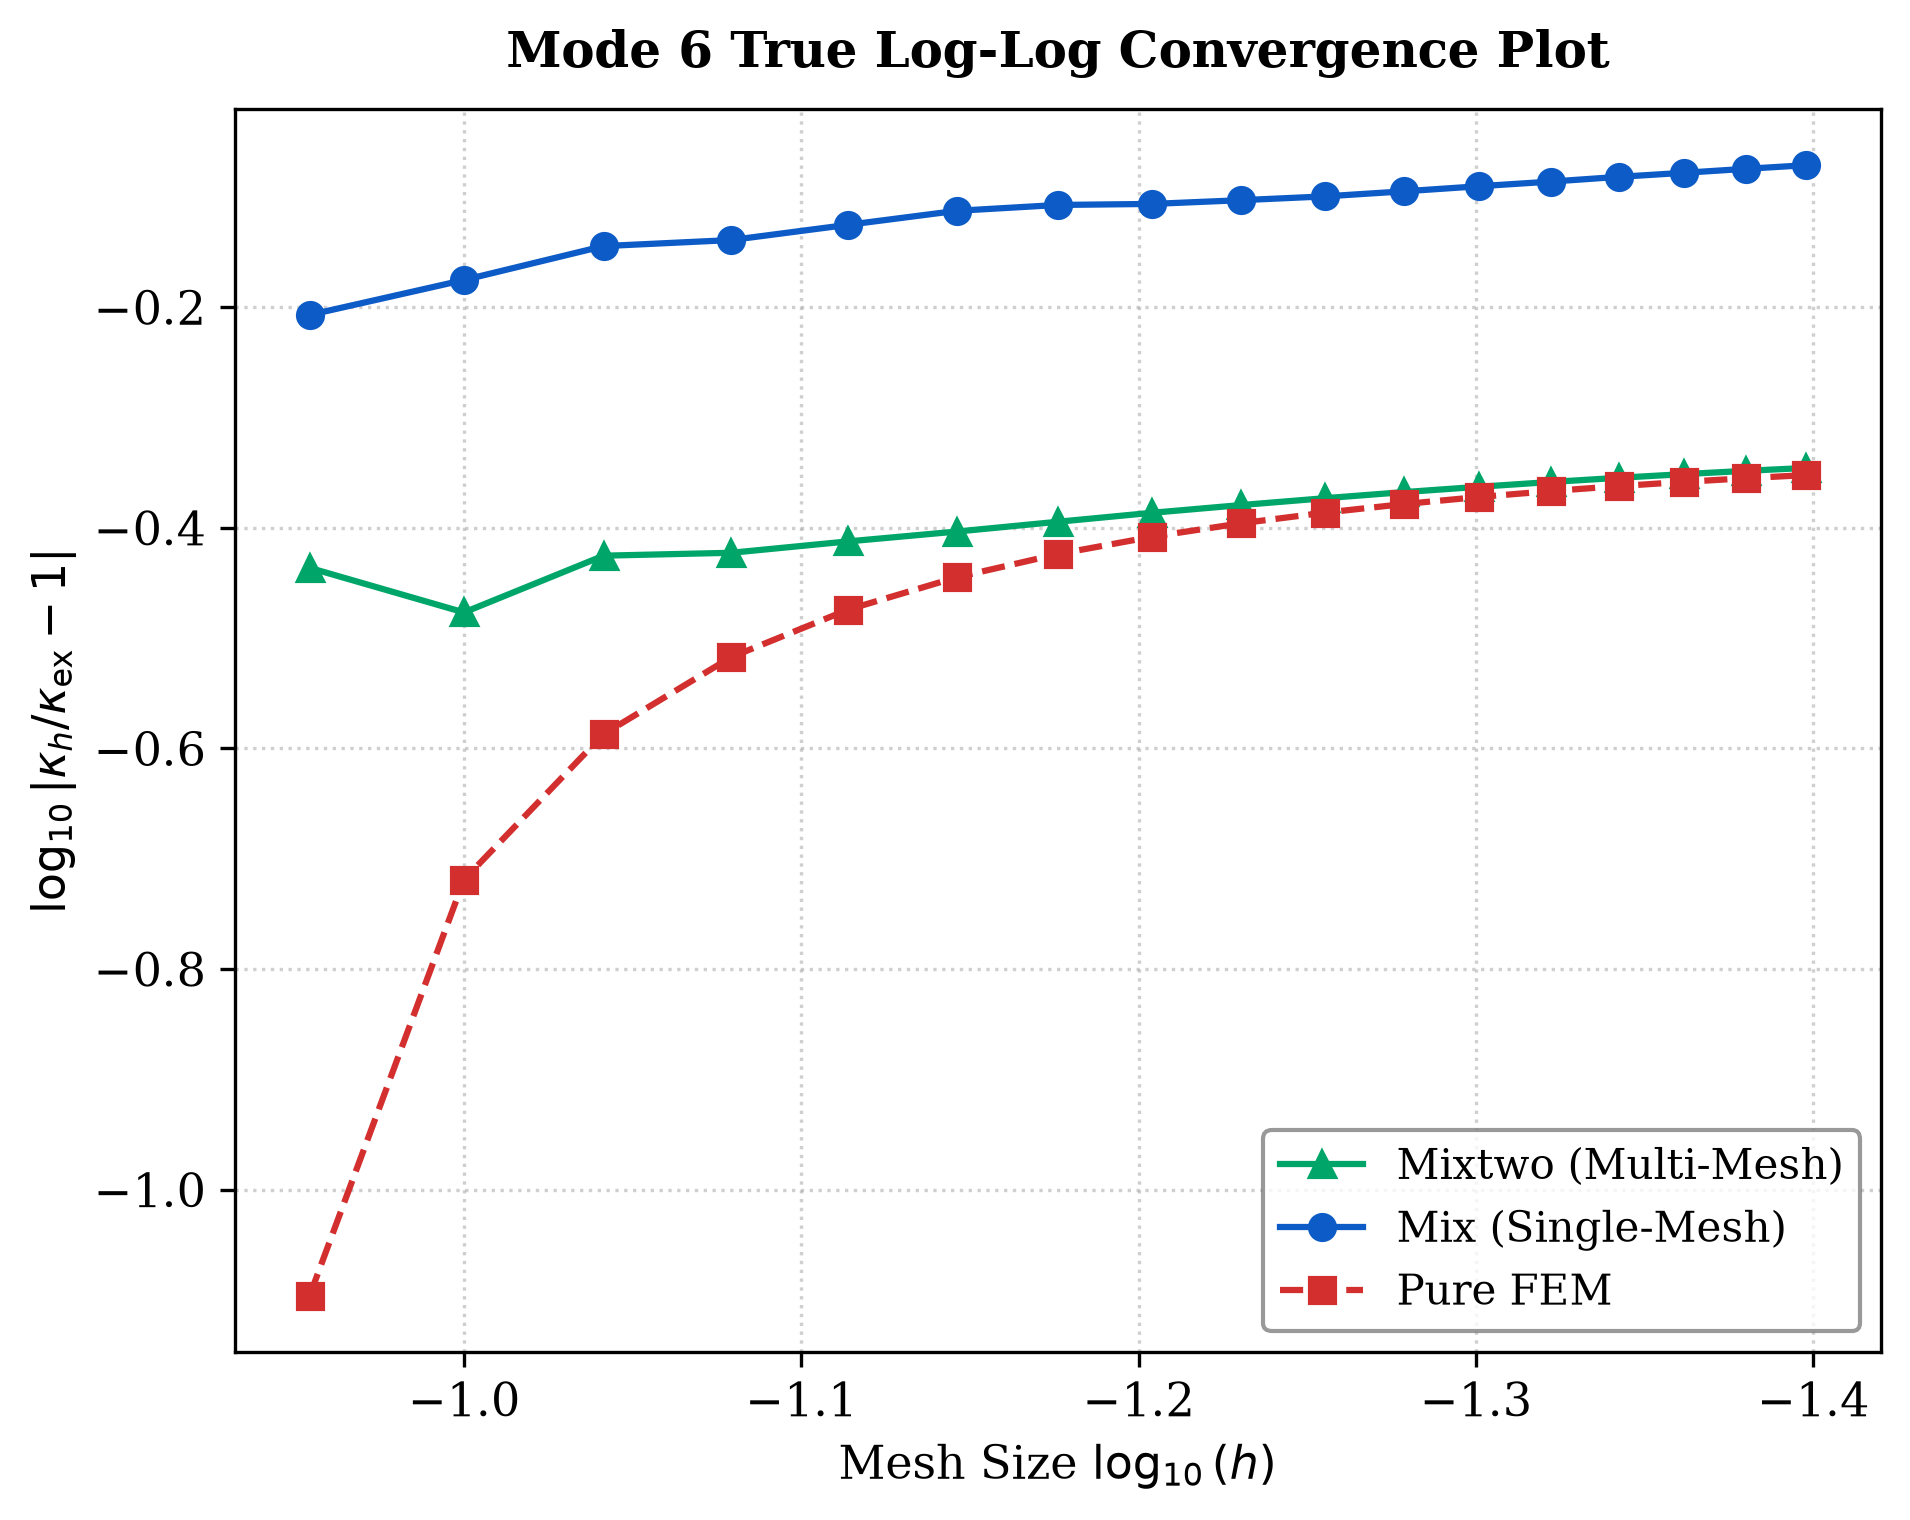
\includegraphics[width=\textwidth]{../images/buckling_mode_6_4c.png}
\caption{模態 6}
\end{subfigure}
\caption{四邊固支板之前六階屈曲模態 (\(h=0.01\))} \label{fig:cccc_modes}
\end{figure}

\subsection{收斂性與誤差分析}
相對誤差同樣定義為
\begin{equation}
\text{Error} = \frac{K_{\text{num}} - K_{\text{ref}}}{K_{\text{ref}}},
\end{equation}
此處 \(K_{\text{ref}}\) 為式 \eqref{eq:K_cccc} 之擬合值（第一模態）或極細網格之收斂值（高階模態）。因 CCCC 板無封閉解析解，主要驗證第一模態的收斂性。

結果顯示，隨著網格加密，第一模態屈曲係數穩定收斂至擬合公式所給之值，驗證了固支邊界處理之正確性。高階模態的數值解亦與古典薄板解趨勢一致（詳見附表）。
